% Original vector reconstruction of source Fig.80.2, PDF325 / printed313.
% Three/four cyclic ribbon ports; arrows are color arrows, not momenta.
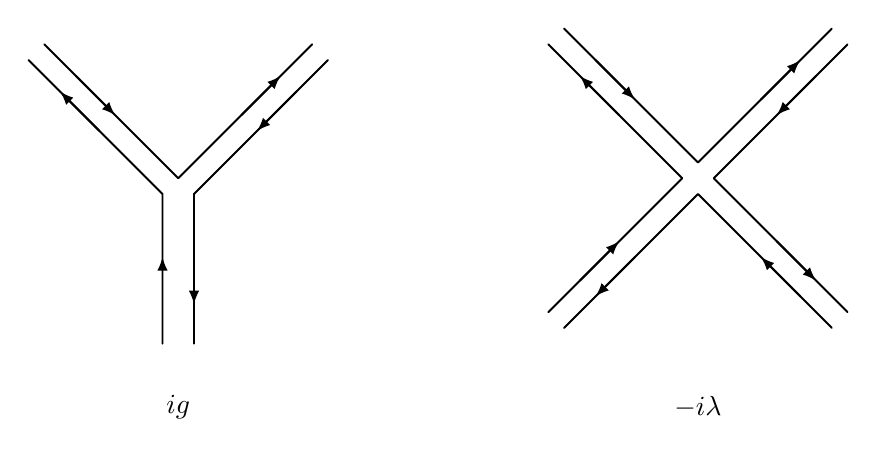
\begin{tikzpicture}[x=1mm,y=1mm,line width=.7pt,>=latex,
 line cap=round,line join=round,font=\fontsize{10}{12}\selectfont]
\begin{scope}[shift={(24,0)}]
  \draw (-17,17)--(0,0)--(17,17);
  \draw (-19,15)--(-2,-2)--(-2,-21);
  \draw (19,15)--(2,-2)--(2,-21);
  \draw[->] (-13,13)--(-8,8);
  \draw[->] (-10,6)--(-15,11);
  \draw[->] (8,8)--(13,13);
  \draw[->] (15,11)--(10,6);
  \draw[->] (-2,-16)--(-2,-10);
  \draw[->] (2,-10)--(2,-16);
  \node at (0,-29) {$ig$};
\end{scope}
\begin{scope}[shift={(90,0)}]
  \draw (-17,19)--(0,2)--(17,19);
  \draw (-19,17)--(-2,0)--(-19,-17);
  \draw (-17,-19)--(0,-2)--(17,-19);
  \draw (19,17)--(2,0)--(19,-17);
  \draw[->] (-13,15)--(-8,10);
  \draw[->] (-10,8)--(-15,13);
  \draw[->] (8,10)--(13,15);
  \draw[->] (15,13)--(10,8);
  \draw[->] (-15,-13)--(-10,-8);
  \draw[->] (-8,-10)--(-13,-15);
  \draw[->] (10,-8)--(15,-13);
  \draw[->] (13,-15)--(8,-10);
  \node at (0,-29) {$-i\lambda$};
\end{scope}
\end{tikzpicture}
